\documentclass{article}
    % General document formatting
    \usepackage[margin=0.7in]{geometry}
    \usepackage[parfill]{parskip}
    \usepackage[utf8]{inputenc}
    \usepackage{amsmath}
    \usepackage{tikz}
    \usepackage{fancyhdr}
    \usepackage{multicol}

    \usetikzlibrary{positioning}

\pagestyle{fancy}
\fancyhf{}
\rhead{Edgar Jacob Rivera Rios - A01184125}

\begin{document}
\section*{2.4.1 First-Order Logic.}
Prove the statements:
\begin{itemize}
    \item $\forall x p ( x ) \wedge \forall x q ( x ) \rightarrow \forall x ( p ( x ) \wedge q ( x ) )$
    \begin{align*}
        A &= \forall xp(x) \wedge \forall x q(x)\\
        B &= \forall x( p(x) \wedge q(x))\\
        A &\rightarrow B
    \end{align*}
    \begin{center}
        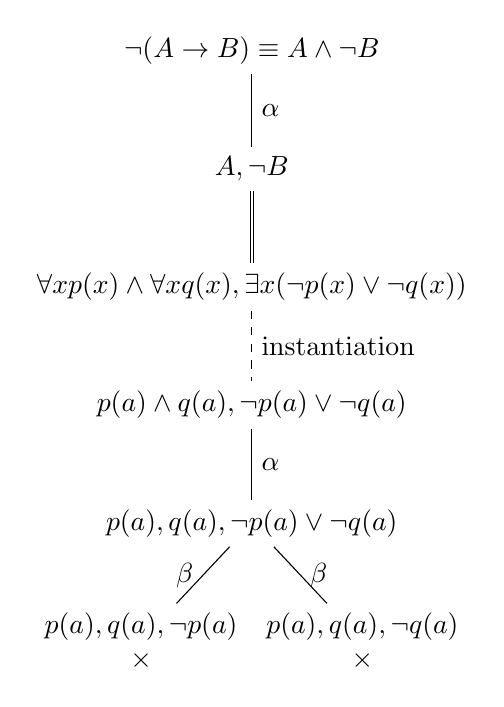
\begin{tikzpicture}[sibling distance=8em, every node/.style = {align=center}]
            \node {$\neg (A \rightarrow B) \equiv A \wedge \neg B$}
            child { node {$A, \neg B$}
              child { node {$\forall xp(x) \wedge \forall x q(x),\exists x (\neg p(x) \vee \neg q(x))$}
                child { node {$p(a) \wedge q(a), \neg p(a) \vee \neg q(a)$}
                  child { node {$p(a), q(a), \neg p(a) \vee \neg q(a)$}
                    child { node {$p(a), q(a), \neg p(a)$\\$\times$}
                      edge from parent node [left] {$\beta$}}
                    child { node {$p(a), q(a), \neg q(a)$\\$\times$}
                      edge from parent node [right] {$\beta$}}
                    edge from parent [solid] node [right] {$\alpha$}}
                  edge from parent [dashed] node [right] {instantiation}}
                edge from parent [double] node {}}
              edge from parent node [right] {$\alpha$}};
        \end{tikzpicture}
    \end{center}
    By contradiction of the inverse we found out that it's valid

    \item $\forall x ( p ( x ) \rightarrow q ( x ) ) \rightarrow ( \forall x p ( x ) \rightarrow \forall x q ( x ) )$ is a valid formula (but its converse $( \forall x p ( x ) \rightarrow \forall x q ( x ) ) \rightarrow \forall x ( p ( x ) \rightarrow q ( x ) )$ is not).
    \begin{align*}
        A &= \forall x(p(x) \rightarrow q(x))\\
        B &= \forall xp(x) \rightarrow \forall x q(x)\\
        A &\rightarrow B
    \end{align*}
    \begin{center}
        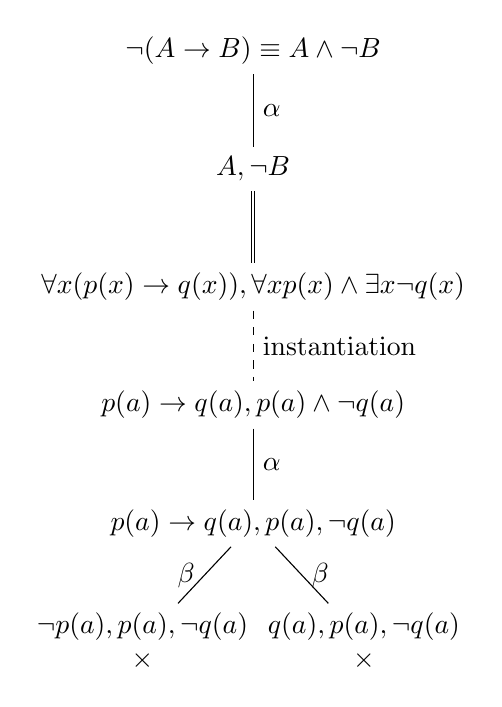
\begin{tikzpicture}[sibling distance=8em, every node/.style = {align=center}]
          \node {$\neg (A \rightarrow B) \equiv A \wedge \neg B$}
            child { node {$A, \neg B$}
              child { node {$\forall x(p(x) \rightarrow q(x)),\forall xp(x) \wedge \exists x \neg q(x)$}
                child { node {$p(a) \rightarrow q(a), p(a) \wedge \neg q(a)$}
                  child { node {$p(a) \rightarrow q(a), p(a), \neg q(a)$}
                    child { node {$\neg p(a) , p(a), \neg q(a)$\\$\times$}
                    edge from parent node [left] {$\beta$}}
                    child { node {$q(a), p(a), \neg q(a)$\\$\times$}
                    edge from parent node [right] {$\beta$}}
                  edge from parent [solid] node [right] {$\alpha$}}
                edge from parent [dashed] node [right] {instantiation}}
              edge from parent [double] node {}}
            edge from parent node [right] {$\alpha$}};
        \end{tikzpicture}
    \end{center}
    By contradiction of the inverse we found out that it's valid
\end{itemize}

\section*{2.4.2 First-Order Logic.}
Prove that the formula $( \forall x p ( x ) \rightarrow \forall x q ( x ) ) \rightarrow \forall x ( p ( x ) \rightarrow q ( x ) )$ is not valid by constructing a semantic tableau for its negation.
\begin{align*}
    A &= \forall xp(x) \rightarrow \forall x q(x) \\
    B &= \forall x(p(x) \rightarrow q(x)) \\
    A &\rightarrow B
\end{align*}
\begin{center}
  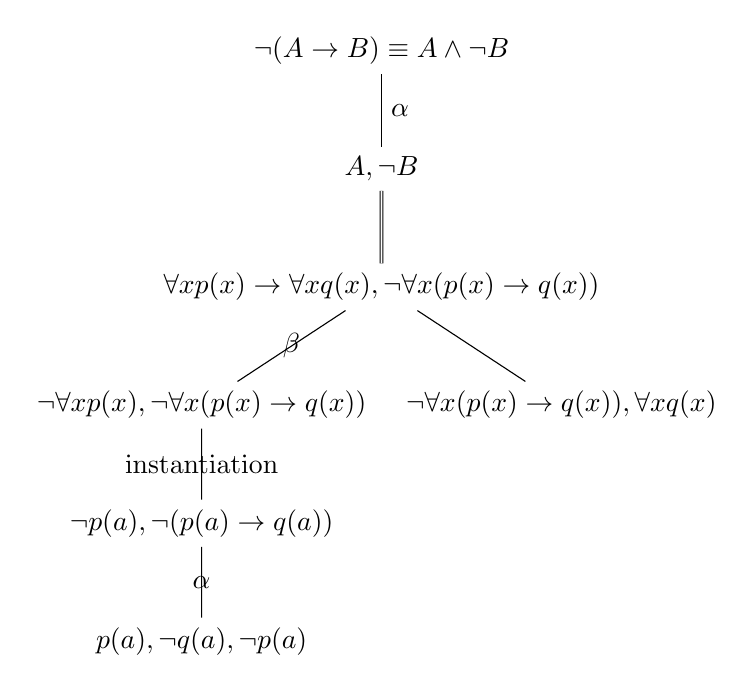
\begin{tikzpicture}[sibling distance=13em, every node/.style = {align=center}]
    \node {$\neg (A \rightarrow B) \equiv A \wedge \neg B$}
      child { node {$A, \neg B$}
        child { node {$\forall xp(x) \rightarrow \forall x q(x), \neg \forall x(p(x) \rightarrow q(x))$}
          child {node {$\neg \forall x p(x), \neg \forall x(p(x) \rightarrow q(x))$}
            child {node {$\neg p(a), \neg (p(a) \rightarrow q(a))$}
              child { node {$p(a), \neg q(a), \neg p(a)$}
              edge from parent node {$\alpha$}}
            edge from parent node {instantiation}}
          edge from parent node {$\beta$}}
          child {node {$\neg \forall x(p(x) \rightarrow q(x)), \forall x q(x)$}}
        edge from parent [double] node {}}
      edge from parent node [right] {$\alpha$}};
  \end{tikzpicture}
\end{center}
\pagebreak
\section*{2.4.3 First-Order Logic.}
Prove that the following formulas are valid
\begin{itemize}
    \item $\exists x (\mathrm { A } ( x ) \rightarrow \mathrm { B } ( x ) ) \leftrightarrow ( \forall x \mathrm { A } ( x ) \rightarrow \exists x \mathrm { B } ( x ) )$
    \begin{align*}
        F &= \exists x (\mathrm { A } ( x ) \rightarrow \mathrm { B } ( x ) ) \\
        G &= ( \forall x \mathrm { A } ( x ) \rightarrow \exists x \mathrm { B } ( x ) )\\
        F &\rightarrow G, G \rightarrow F
    \end{align*}
    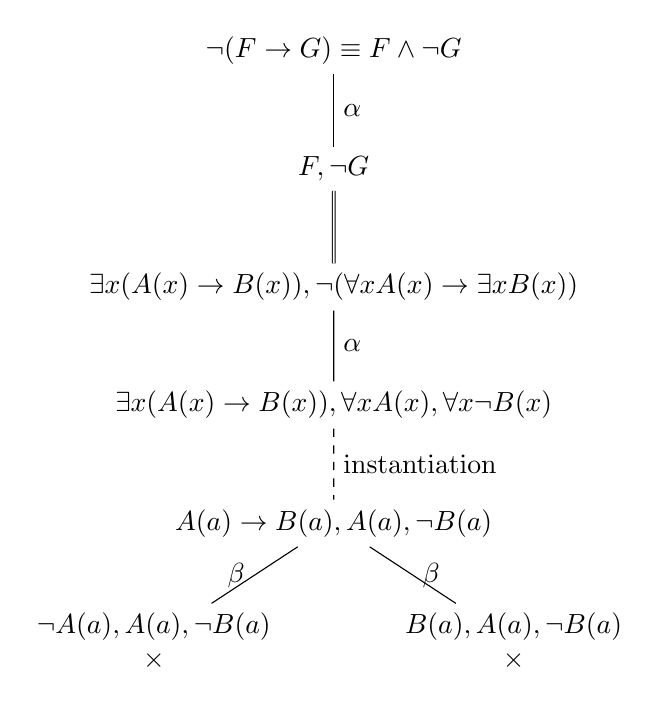
\begin{tikzpicture}[sibling distance=13em, every node/.style = {align=center}]
      \node {$\neg (F \rightarrow G) \equiv F \wedge \neg G$}
        child { node {$F, \neg G$}
          child { node {$\exists x(A(x) \rightarrow B(x)), \neg (\forall x A(x) \rightarrow \exists x B(x))$}
            child { node {$\exists x(A(x) \rightarrow B(x)),\forall x A(x), \forall x \neg B(x)$}
              child { node {$A(a) \rightarrow B(a), A(a), \neg B(a)$}
                child { node {$\neg A(a), A(a), \neg B(a)$\\$\times$}
                edge from parent [solid] node [left] {$\beta$}}
                child { node {$B(a), A(a), \neg B(a)$\\$\times$}
                edge from parent [solid] node [right] {$\beta$}}
              edge from parent [dashed] node [right] {instantiation}}
            edge from parent node [right] {$\alpha$}}
          edge from parent [double] node {}}
        edge from parent node [right] {$\alpha$}};
    \end{tikzpicture}
    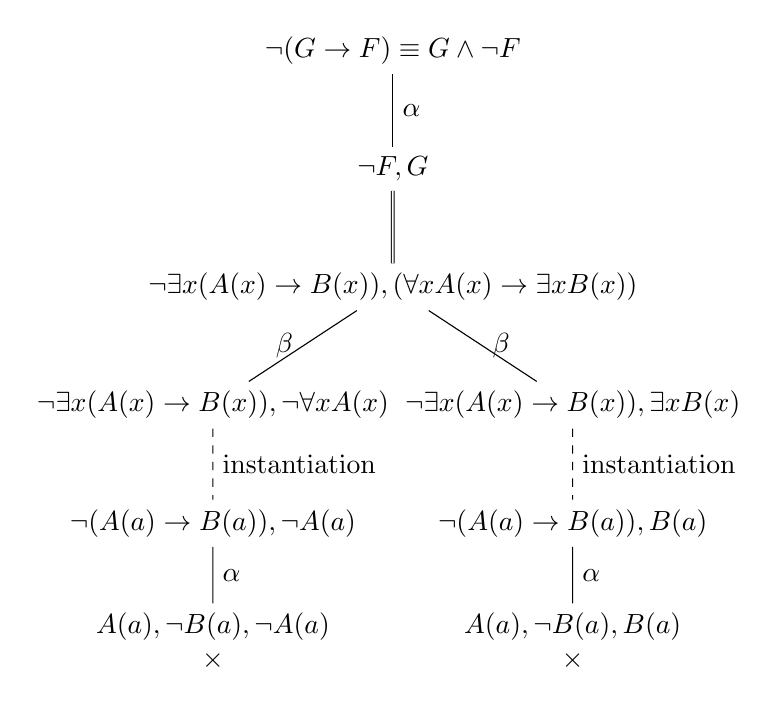
\begin{tikzpicture}[sibling distance=13em, every node/.style = {align=center}]
      \node {$\neg (G \rightarrow F) \equiv G \wedge \neg F$}
        child { node {$\neg F, G$}
          child { node {$ \neg \exists x(A(x) \rightarrow B(x)), (\forall x A(x) \rightarrow \exists x B(x))$}
            child { node {$\neg \exists x(A(x) \rightarrow B(x)), \neg \forall x A(x)$}
              child { node {$\neg (A(a) \rightarrow B(a)), \neg A(a)$}
                child { node {$A(a), \neg B(a), \neg A(a)$\\$\times$}
                edge from parent [solid] node [right] {$\alpha$}}
              edge from parent [dashed] node [right] {instantiation}}
            edge from parent node [left] {$\beta$}}
            child { node {$\neg \exists x(A(x) \rightarrow B(x)), \exists x B(x)$}
              child { node {$\neg (A(a) \rightarrow B(a)), B(a)$}
                child { node {$A(a), \neg B(a), B(a)$\\$\times$}
                edge from parent [solid] node [right] {$\alpha$}}
              edge from parent [dashed] node [right] {instantiation}}
            edge from parent node [right] {$\beta$}}
          edge from parent [double] node {}}
        edge from parent node [right] {$\alpha$}};
    \end{tikzpicture}\\
    It's true by contradiction of the inverse implications
    \item $(\exists x A(x) \rightarrow \forall x B(x)) \rightarrow \forall x(A(x) \rightarrow B(x))$
    \item $\forall x (A(x) \vee B(x)) \rightarrow (\forall x A(x) \vee \exists x B(x))$
    \item $\forall x (A(x) \rightarrow B(x)) \rightarrow (\exists x A(x) \rightarrow \exists x B(x))$
\end{itemize}
\end{document}